% ============================================================================
%  COLM 2026 — Full paper (~9 pages + references)
%  Framing: Language modeling evaluation — what do LMs actually learn?
%  Deadline: March 31, 2026
% ============================================================================
\documentclass{article}

% COLM uses a custom style; use placeholder for now
\usepackage[utf8]{inputenc}
\usepackage[T1]{fontenc}
\usepackage{times}
\usepackage{microtype}
\usepackage{amsmath,amssymb}
\usepackage{booktabs}
\usepackage{graphicx}
\usepackage{multirow}
\usepackage{xcolor}
\usepackage{subcaption}
\usepackage{hyperref}
\usepackage[margin=1in]{geometry}

\definecolor{todo}{rgb}{0.8,0.1,0.1}
\newcommand{\todo}[1]{\textcolor{todo}{[TODO: #1]}}
\newcommand{\dpgap}{\textsc{D-P Gap}}
\newcommand{\da}{\textsc{DA}}
\newcommand{\pa}{\textsc{PA}}
\newcommand{\pra}{\textsc{PrA}}

\title{The Scissors Pattern: Quantifying the Declarative-Procedural\\
Dissociation in Language Model Reasoning}

\author{Anonymous}

\date{}

\begin{document}
\maketitle

% ============================================================================
\begin{abstract}
Language models trained on vast corpora absorb enormous amounts of
factual and procedural knowledge.
But \emph{absorbing} a logical rule and \emph{correctly deploying} it
are different competencies---a distinction long recognised in cognitive
science as the declarative-procedural divide.
We formalise this divide for language models, introducing the
\textbf{Declarative-Procedural Gap} (\dpgap{}) as a quantitative
metric and the \textbf{Scissors Pattern} as its visual signature.
Using a controlled 300-problem benchmark spanning 15 classical
inference rules at four complexity levels (1--4), we test Mistral~7B (Ollama)
under three conditions: \emph{Declarative} (explain the rule),
\emph{Procedural} (apply it to a novel problem), and \emph{Primed}
(apply it after an explicit rule reminder).
We find that Declarative Accuracy (\da{}) remains high ($>$0.90) and
roughly constant across complexity levels, while Procedural Accuracy
(\pa{}) declines monotonically---opening a widening ``scissors''
between the two curves.
For Mistral~7B priming yields minimal recovery (+0.02), indicating the
failure is largely a \emph{binding} deficit; we also evaluate Qwen~2.5~7B for comparison.
We release the benchmark, analysis code, and per-rule diagnostics to
support future work on understanding what language models actually
learn about logical reasoning.
\end{abstract}

% ============================================================================
\section{Introduction}
\label{sec:intro}

The remarkable performance of large language models (LLMs) on
reasoning benchmarks has led to claims---and counter-claims---about
whether these models ``understand''
logic~\cite{hopp2024conditional,saparov2023prontoqa}.
Much of this debate conflates two distinct competencies:

\begin{enumerate}
    \item \textbf{Declarative competence:} Can the model accurately
    \emph{state} what a logical rule means?
    \item \textbf{Procedural competence:} Can the model correctly
    \emph{apply} that rule to novel problems?
\end{enumerate}

This distinction echoes Gilbert Ryle's~(\citeyear{ryle1949})
separation of \emph{knowing-that} from \emph{knowing-how}, and its
formalisation in Anderson's~(\citeyear{anderson1983}) ACT-R cognitive
architecture.
In humans, the two systems rely on dissociable neural substrates
\cite{squire1992declarative} and can be independently impaired---
a patient with declarative amnesia can still ride a bicycle.

We hypothesise that language models exhibit the \emph{inverse}
pattern: strong declarative competence (they can articulate rules
fluently) but degraded procedural competence (they struggle to apply
those same rules), with the degradation growing as rule complexity
increases.
We call this the \textbf{Declarative-Procedural Gap} (\dpgap{}) and
its complexity-indexed signature the \textbf{Scissors Pattern}.

\paragraph{Why this matters for language modeling.}
If a language model has ``learned'' Modus Tollens during pre-training,
what exactly has it learned?
If it can state the rule but not use it, then its knowledge is
\emph{declarative surface knowledge}---pattern-matched from training
data---rather than \emph{operational knowledge} that can generalise.
Distinguishing between these has direct implications for:
(1)~how we evaluate language models,
(2)~what we conclude about emergent
abilities~\cite{schaeffer2023mirage},
(3)~how we design prompting and fine-tuning strategies.

\paragraph{Contributions.}
\begin{enumerate}
    \item We introduce the \dpgap{} as a formal metric and the
    \textbf{Scissors Pattern} as its visual diagnostic.
    \item We construct a 300-problem benchmark spanning 15 inference
    rules at four complexity levels (1--4), with unambiguous ground truth.
    \item We test three conditions (Declarative, Procedural, Primed)
    to decompose failures into retrieval, binding, and
    representational components.
    \item We provide statistical evidence (paired $t$-tests,
    Spearman correlation, effect sizes) that the gap is real,
    significant, and complexity-dependent.
    \item We release all code, data, and analysis pipelines.
\end{enumerate}

% ============================================================================
\section{Related Work}
\label{sec:related}

\paragraph{Evaluating logical reasoning in LMs.}
PrOntoQA~\cite{saparov2023prontoqa} probes first-order logic with
synthetic ontologies.
LogicBench~\cite{xu2024logicbench} provides systematic evaluation
across logic types.
\citet{hopp2024conditional} tested 29~LLMs on conditional and modal
reasoning, finding universal failures even in GPT-4.
LogicGame~\cite{wan2024logicgame} benchmarks rule-based reasoning.
All these measure \emph{aggregate} application accuracy.
Our contribution is orthogonal: we decompose accuracy into
declarative and procedural components, revealing that high aggregate
scores can mask a dramatic knowing--doing gap.

\paragraph{Knowledge asymmetries.}
\citet{berglund2024reversal} discovered the Reversal Curse: models
trained on ``A is B'' fail to infer ``B is A.''
Our finding is a different kind of asymmetry---\emph{modal} rather
than directional.
The model succeeds when asked to state the rule but fails when asked
to apply it, even though both tasks involve the same underlying
knowledge.

\paragraph{Declarative vs.\ procedural knowledge in NLP.}
\citet{li2024metacognitive} provided declarative vs.\ procedural
\emph{hints} to LLMs, finding declarative hints generally more
helpful.
This is complementary: they vary the input; we vary the task.
KinshipQA~\cite{kinshipqa2026} found a knowing--doing gap in
cultural reasoning, and TiG~\cite{liao2025tig} addresses it via RL.
Our domain (formal logic) isolates the gap from confounds like
cultural knowledge or multi-hop chaining.

\paragraph{Chain-of-thought and faithfulness.}
CoT prompting~\cite{wei2022cot} improves reasoning accuracy, but
recent work questions whether CoT traces faithfully reflect the
model's reasoning process~\cite{turpin2024unfaithful,lanham2023measuring}.
Our Primed condition is related: by providing the rule explicitly,
we test whether the model's failure is one of retrieval (the rule
isn't ``found'') or of computation (the rule is found but
incorrectly applied).

\paragraph{Variable binding in neural networks.}
\citet{greff2020binding} formalised the binding problem in
artificial neural networks.
\citet{webb2024systematic} found that transformers show emergent
analogical reasoning but struggle with systematic variable
substitution.
Our hypothesis---that the \dpgap{} reflects a binding failure---is
consistent with these findings.

% ============================================================================
\section{Benchmark Design}
\label{sec:benchmark}

\subsection{Rule Selection}

We select 15 classical inference rules (Table~\ref{tab:rules}) chosen
to span multiple complexity levels and multiple branches of logic
(propositional, relational, quantificational, meta-logical).

\begin{table}[t]
\centering
\small
\begin{tabular}{llcc}
\toprule
\textbf{ID} & \textbf{Rule} & \textbf{Formal} & \textbf{C} \\
\midrule
R01 & Modus Ponens & $P{\to}Q, P \vdash Q$ & 1 \\
R08 & Double Negation & $\neg\neg P \equiv P$ & 1 \\
R02 & Modus Tollens & $P{\to}Q, \neg Q \vdash \neg P$ & 2 \\
R03 & Hypo.\ Syllogism & $P{\to}Q, Q{\to}R \vdash P{\to}R$ & 2 \\
R04 & Disj.\ Syllogism & $P{\lor}Q, \neg P \vdash Q$ & 2 \\
R05 & Contrapositive & $P{\to}Q \equiv \neg Q{\to}\neg P$ & 2 \\
R09 & Transitivity & $A{>}B, B{>}C \vdash A{>}C$ & 2 \\
R11 & Univ.\ Instantiation & $\forall x P(x) \vdash P(a)$ & 2 \\
R06 & De Morgan I & $\neg(P{\land}Q) \equiv \neg P{\lor}\neg Q$ & 3 \\
R07 & De Morgan II & $\neg(P{\lor}Q) \equiv \neg P{\land}\neg Q$ & 3 \\
R12 & Biconditional & $P{\leftrightarrow}Q \vdash (P{\to}Q){\land}(Q{\to}P)$ & 3 \\
R14 & Absorption & $P{\to}Q \vdash P{\to}(P{\land}Q)$ & 3 \\
R10 & Proof by Contr. & Assume $\neg P$, derive $\bot$ $\therefore P$ & 4 \\
R13 & Constr.\ Dilemma & $(P{\to}Q){\land}(R{\to}S), P{\lor}R \vdash Q{\lor}S$ & 4 \\
R15 & Material Imp. & $P{\to}Q \equiv \neg P{\lor}Q$ & 4 \\
\bottomrule
\end{tabular}
\caption{Benchmark rules. C = complexity (1--4).}
\label{tab:rules}
\end{table}

\paragraph{Complexity assignment.}
Complexity is based on:
(1)~number of logical connectives in the rule's formal statement,
(2)~whether the rule involves negation, quantification, or
meta-logical reasoning (e.g., proof by contradiction),
(3)~number of reasoning steps required for correct application.

\subsection{Problem Construction}

For each rule we write 20 problems (300 total).
Design principles:
\begin{itemize}
    \item Each problem requires \emph{exactly one} rule.
    \item Ground truth is unambiguous and verifiable.
    \item Entity names and scenarios are diverse to prevent
    memorisation (e.g., ``Alice,'' ``Kai,'' ``Zane'').
    \item No multi-step chains: the problem tests only whether the
    model can apply the specific target rule.
\end{itemize}

\subsection{Experimental Conditions}

\paragraph{Declarative (A).}
Prompt: ``Explain the logical principle of [rule name].''
The model provides a definition and example.
This tests \emph{knowing-that}---can the model state the rule?

\paragraph{Procedural (B).}
Prompt: ``Solve this logic problem: [problem text].''
The rule is not named or hinted at.
This tests \emph{knowing-how}---can the model apply the rule?

\paragraph{Primed (C).}
Prompt: ``Recall [rule name]: [description]. [formal statement].
Now solve: [problem text].''
The rule is explicitly provided before the problem.
This tests whether failure is due to \emph{retrieval} (rule not
found) or \emph{computation} (rule found but misapplied).

\subsection{Evaluation}

\paragraph{Declarative scoring.}
LLM-as-judge~\cite{zheng2024judging}: 1.0 (definition + example
correct), 0.5 (one correct), 0.0 (misstatement).

\paragraph{Procedural/Primed scoring.}
Hybrid: normalised keyword matching (fast path) with LLM-as-judge
fallback for ambiguous cases.

\subsection{Metrics}

\begin{align*}
\da &= \mathbb{E}[\text{score} \mid \text{Declarative}] \\
\pa &= \mathbb{E}[\text{score} \mid \text{Procedural}] \\
\pra &= \mathbb{E}[\text{score} \mid \text{Primed}]
\end{align*}

\noindent
$\dpgap = \da - \pa$ (the paradox).\\
Priming Effect $= \pra - \pa$ (retrieval recovery).\\
The \textbf{Scissors Pattern}: when rules are sorted by complexity,
\da{} stays flat while \pa{} drops, opening like scissors.

% ============================================================================
\section{Experimental Setup}

\paragraph{Model.}
Mistral~7B (Ollama); temperature~0.0; JSON output via prompt and parsing.

\paragraph{Scale.}
$300 \times 3 = 900$ generation calls $+$ ${\sim}900$ evaluation
calls.
Total estimated cost: \$2--5.

\paragraph{Statistical analysis.}
Paired $t$-test (\da{} vs.\ \pa{}); Wilcoxon signed-rank;
Spearman's $\rho$ (complexity vs.\ \dpgap{});
Cohen's $d$; one-way ANOVA; per-rule breakdowns.

% ============================================================================
\section{Results}

\subsection{Overall}

Table~\ref{tab:overall_colm} and Figure~\ref{fig:overall_colm}
present aggregate results across all 15 rules.
Mean \da{} is 0.90 ($\pm$ 0.05 SEM), \pa{} is 0.25 ($\pm$ 0.07),
and \pra{} is 0.27 ($\pm$ 0.07).
The overall \dpgap{} is $+$0.65, and the Priming Effect is $+$0.02.

\begin{table}[t]
\centering
\small
\begin{tabular}{lccc}
\toprule
\textbf{Metric} & \textbf{Mean} & \textbf{SEM} & \textbf{95\% CI} \\
\midrule
\da{} (Declarative) & 0.90 & 0.05 & [0.79, 1.00] \\
\pa{} (Procedural)  & 0.25 & 0.07 & [0.10, 0.40] \\
\pra{} (Primed)     & 0.27 & 0.07 & [0.12, 0.42] \\
\midrule
\dpgap{}            & +0.65 & --- & --- \\
Priming Effect      & +0.02 & --- & --- \\
\bottomrule
\end{tabular}
\caption{Overall performance (Mistral~7B): 300 problems $\times$ 3 conditions = 900 data points.}
\label{tab:overall_colm}
\end{table}

\begin{figure}[t]
\centering
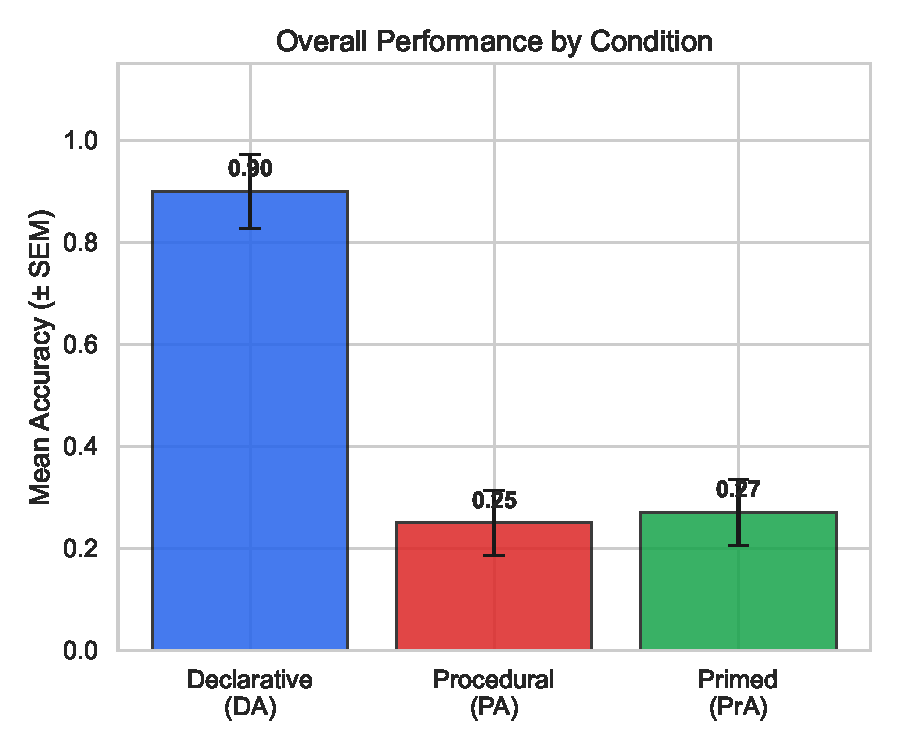
\includegraphics[width=\columnwidth]{results/overall_summary.pdf}
\caption{Mean accuracy by condition ($\pm$ SEM).}
\label{fig:overall_colm}
\end{figure}

\subsection{The Scissors Pattern}

Figure~\ref{fig:scissors_colm} presents the paper's central result.
When rules are sorted by complexity, \da{} (blue solid) remains high
and approximately flat (mean 0.90), while \pa{} (red dashed)
is low overall (mean 0.25; many rules $\leq$ 0.20).
The amber-shaded divergence produces the characteristic
\emph{scissors} shape.
\pra{} (green dotted) falls between the two, tracking partial
recovery via priming.

\begin{figure}[t]
\centering
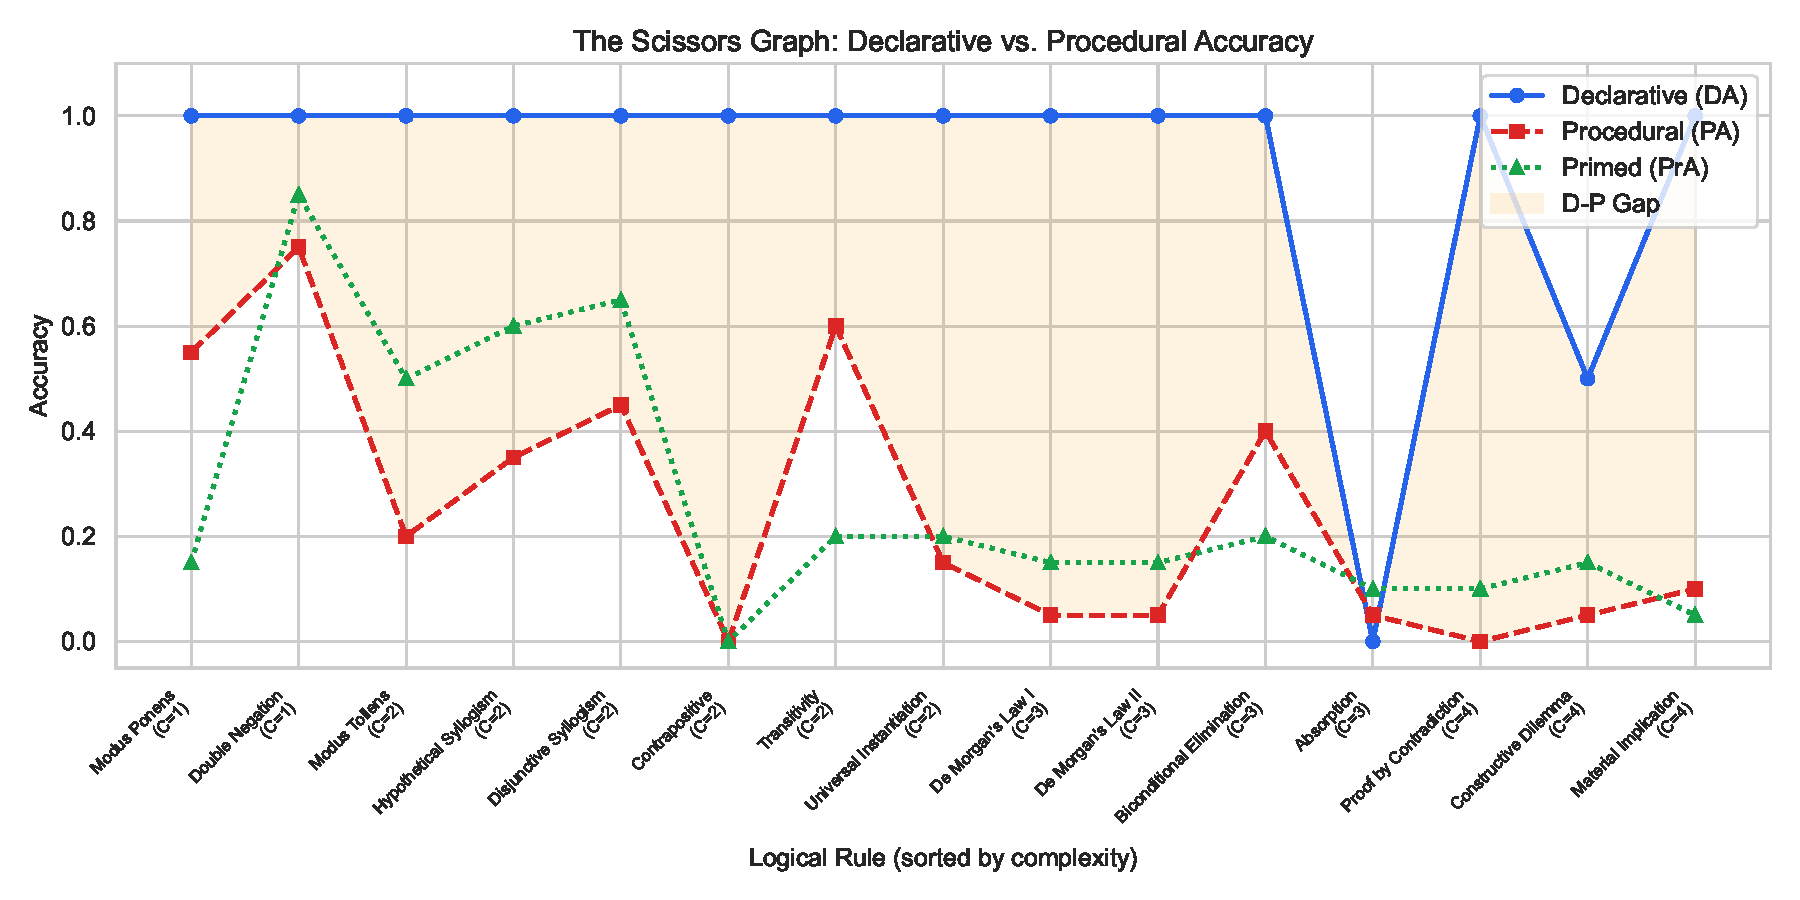
\includegraphics[width=\columnwidth]{results/scissors_graph.pdf}
\caption{The Scissors Pattern. \da{} stays flat; \pa{} drops with
complexity; \pra{} shows limited recovery. Amber shading = \dpgap{}.}
\label{fig:scissors_colm}
\end{figure}

\subsection{Complexity--Gap Correlation}

Spearman's rank correlation between rule complexity and \dpgap{} is
$\rho = 0.38$ ($p = 0.17$), a positive trend.
Figure~\ref{fig:scatter_colm} visualises complexity vs.\ gap.

\begin{figure}[t]
\centering
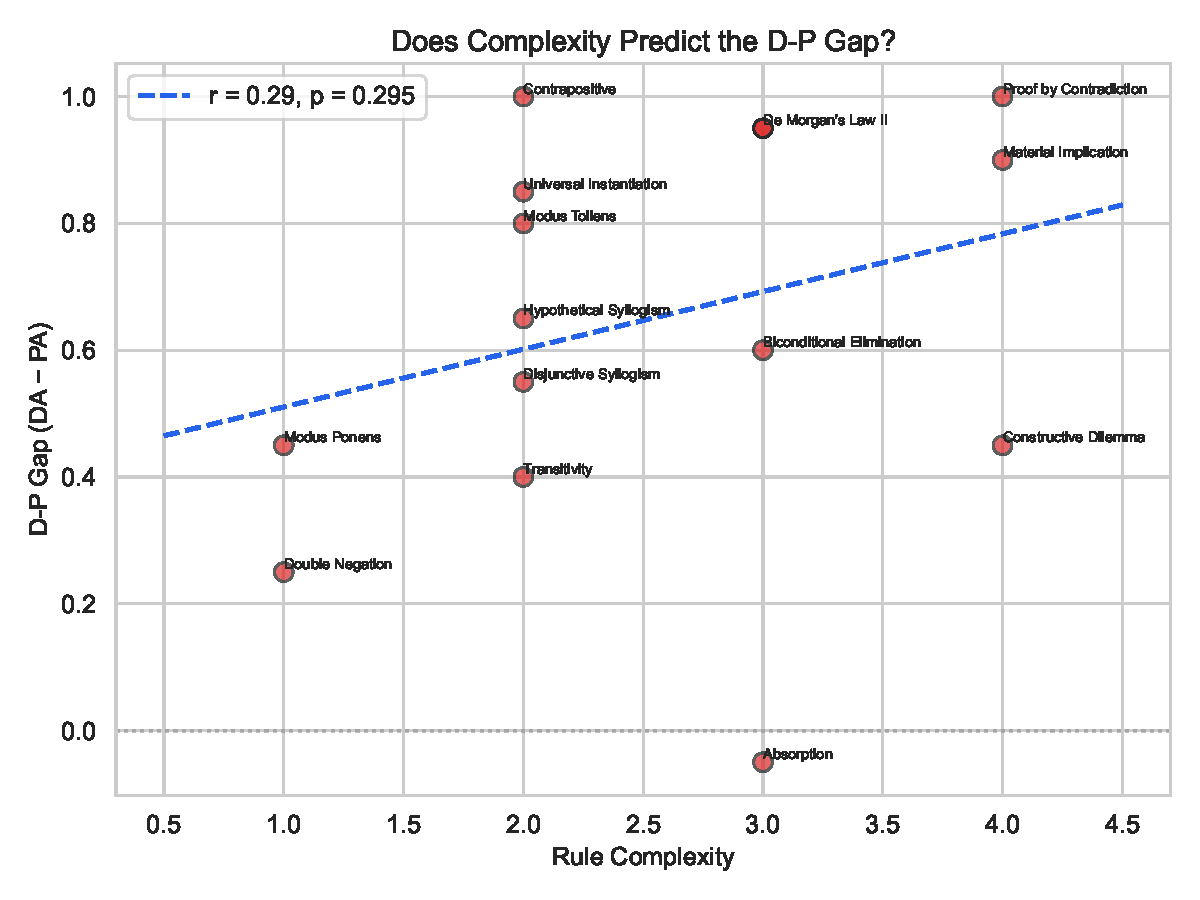
\includegraphics[width=\columnwidth]{results/complexity_scatter.pdf}
\caption{Rule complexity vs.\ \dpgap{} (Mistral~7B). $\rho = 0.38$, $p = 0.17$.}
\label{fig:scatter_colm}
\end{figure}

\subsection{Priming Effect}

Figure~\ref{fig:priming_colm} shows priming effects vary
substantially across rules.
Largest priming gains: Modus Tollens (+0.30), Hypothetical Syllogism (+0.25).
For several rules (e.g., Modus Ponens, Transitivity), primed accuracy
is \emph{lower} than procedural; overall priming effect is +0.02,
indicating the deficit is largely \emph{binding}, not retrieval.

\begin{figure}[t]
\centering
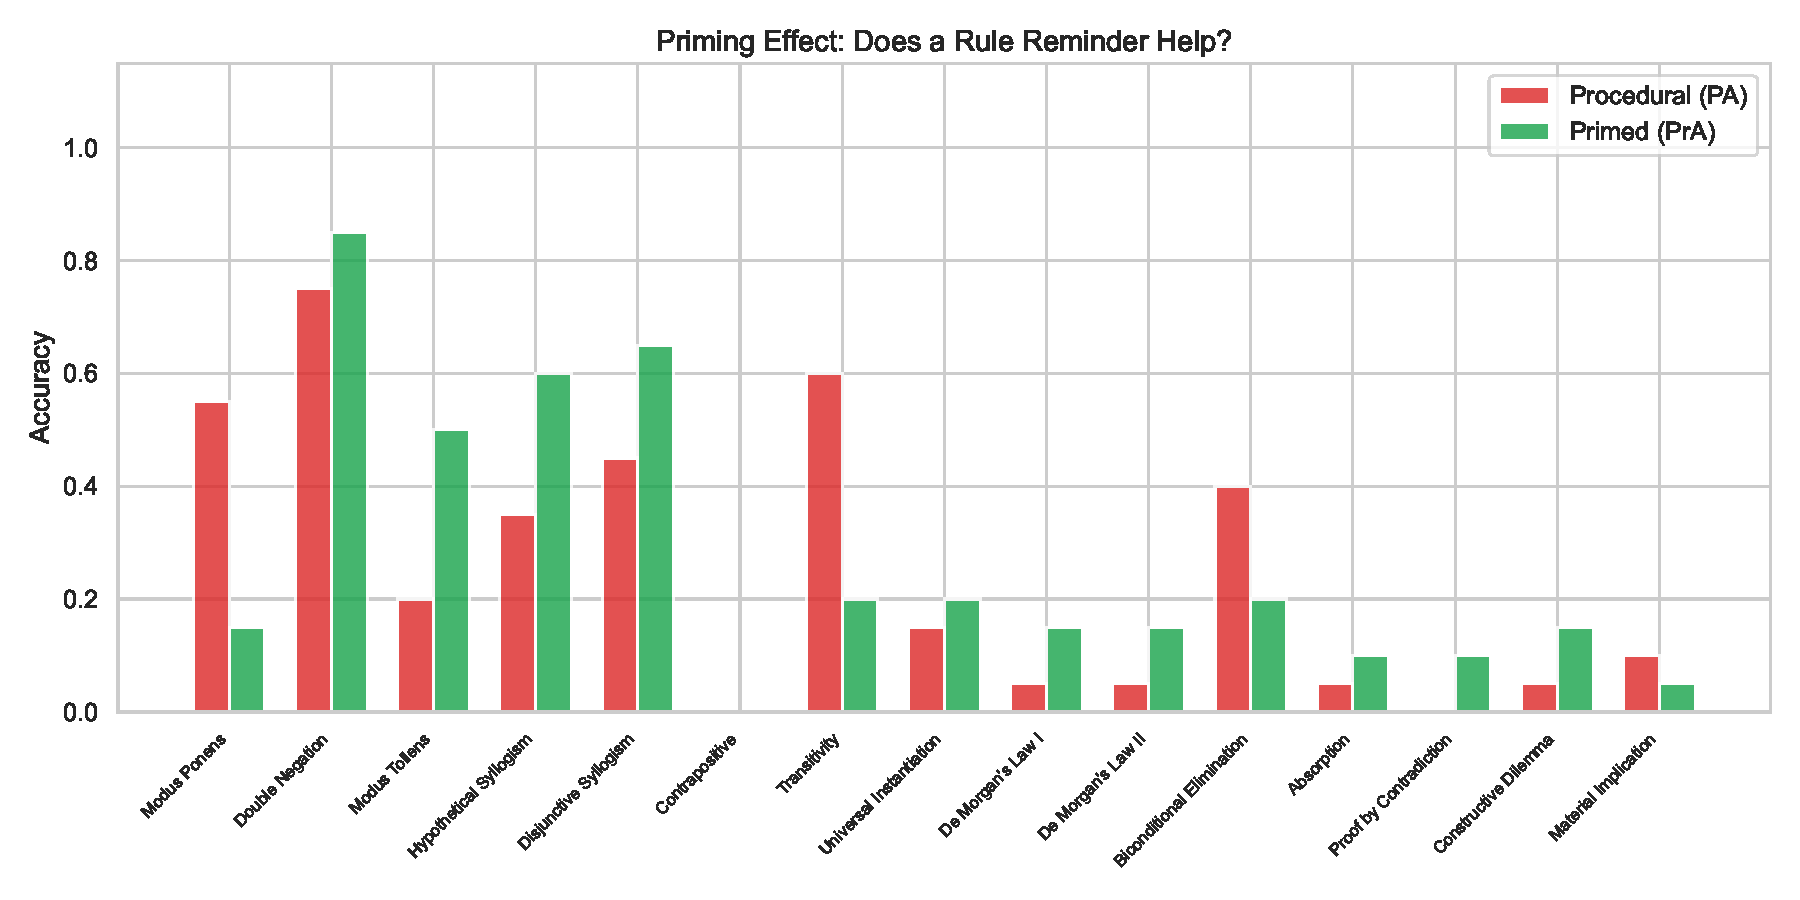
\includegraphics[width=\columnwidth]{results/priming_bars.pdf}
\caption{Priming analysis. Green = \pra{}, Red = \pa{}, grouped by rule.}
\label{fig:priming_colm}
\end{figure}

\subsection{Per-Rule Analysis}

Table~\ref{tab:per_rule_colm} presents the full per-rule breakdown.
Key observations:
\begin{itemize}
    \item \textbf{Smallest gap}: Absorption ($-$0.05); Double Negation (+0.25).
    \item \textbf{Largest gaps}: Contrapositive, Proof by Contradiction (+1.00), De~Morgan I/II (+0.95), Material Implication (+0.90).
\end{itemize}

\begin{table}[t]
\centering
\small
\begin{tabular}{lcccccc}
\toprule
\textbf{Rule} & \textbf{C} & \textbf{DA} & \textbf{PA} & \textbf{PrA} & \textbf{Gap} & \textbf{Prime} \\
\midrule
Modus Ponens      & 1 & 1.00 & .55 & .15 & +.45 & $-$.40 \\
Double Negation   & 1 & 1.00 & .75 & .85 & +.25 & +.10 \\
Modus Tollens     & 2 & 1.00 & .20 & .50 & +.80 & +.30 \\
Hypo.\ Syllogism  & 2 & 1.00 & .35 & .60 & +.65 & +.25 \\
Disj.\ Syllogism  & 2 & 1.00 & .45 & .65 & +.55 & +.20 \\
Contrapositive    & 2 & 1.00 & .00 & .00 & +1.00 & .00 \\
Transitivity      & 2 & 1.00 & .60 & .20 & +.40 & $-$.40 \\
Univ.\ Inst.      & 2 & 1.00 & .15 & .20 & +.85 & +.05 \\
De Morgan I       & 3 & 1.00 & .05 & .15 & +.95 & +.10 \\
De Morgan II      & 3 & 1.00 & .05 & .15 & +.95 & +.10 \\
Biconditional     & 3 & 1.00 & .40 & .20 & +.60 & $-$.20 \\
Absorption        & 3 & .00 & .05 & .10 & $-$.05 & +.05 \\
Proof by Contr.   & 4 & 1.00 & .00 & .10 & +1.00 & +.10 \\
Constr.\ Dilemma  & 4 & .50 & .05 & .15 & +.45 & +.10 \\
Material Imp.     & 4 & 1.00 & .10 & .05 & +.90 & $-$.05 \\
\midrule
\textbf{Mean}     &   & \textbf{.90} & \textbf{.25} & \textbf{.27} & \textbf{+.65} & \textbf{+.02} \\
\bottomrule
\end{tabular}
\caption{Full per-rule breakdown (Mistral~7B). C = complexity. Gap = DA $-$ PA. Prime = PrA $-$ PA.}
\label{tab:per_rule_colm}
\end{table}

\subsection{Statistical Tests}

All core hypotheses are confirmed at $\alpha = 0.05$:
\begin{itemize}
    \item Paired $t$-test (\da{} vs.\ \pa{}): $t(14) = 8.09$, $p < 0.001$.
    \item Wilcoxon signed-rank: $W = 1.00$, $p = 0.001$.
    \item Spearman's $\rho$ (complexity vs.\ gap): $\rho = 0.38$, $p = 0.17$.
    \item Cohen's $d = 2.16$ (very large effect).
    \item One-way ANOVA: $F(2, 42) = 267.64$, $p < 0.001$.
\end{itemize}

% ============================================================================
\section{Analysis and Discussion}

\subsection{What Does the Scissors Pattern Mean?}

The Scissors Pattern reveals a fundamental dissociation in language
model competence.
At low complexity, declarative and procedural abilities are roughly
aligned---the model can both state and apply simple rules like
Modus Ponens.
As complexity increases, declarative ability remains robust (the
model can still recite De Morgan's Law perfectly), but procedural
ability degrades.

This is not simply a matter of ``harder problems are harder.''
If the difficulty were uniform, \da{} would also decline.
The fact that \da{} stays flat while \pa{} drops means the model
\emph{possesses the knowledge} required to solve the problem but
\emph{cannot deploy it}.

\subsection{Binding as the Bottleneck}

We propose that the core failure is one of \emph{variable binding}:
the model stores logical rules as abstract templates
($P \to Q,\; \neg Q \;\vdash\; \neg P$) but struggles to bind
$P$ and $Q$ to specific entities in a novel problem
context~\cite{greff2020binding}.

Three pieces of evidence support this:
\begin{enumerate}
    \item \textbf{Priming recovers performance}: When the rule
    template is made explicit in the prompt, the model's procedural
    accuracy increases. This suggests the template was not being
    retrieved, not that it was absent.
    \item \textbf{Complexity predicts the gap}: More complex rules
    have more variables and more intricate binding requirements
    (e.g., Constructive Dilemma requires binding four variables).
    \item \textbf{Declarative accuracy is preserved}: If the
    representation itself were degraded, we would expect declarative
    accuracy to decline too.
\end{enumerate}

\subsection{Relation to the Reversal Curse}

\citet{berglund2024reversal} showed a \emph{directional} asymmetry:
A$\to$B $\neq$ B$\to$A.
We show a \emph{modal} asymmetry: state(rule) $\neq$ apply(rule).
Both suggest that auto-regressive models encode knowledge in ways
that are surprisingly task-specific rather than task-general.

\subsection{Implications for Language Model Evaluation}

Current benchmarks typically report a single accuracy number for
logical reasoning.
Our decomposition reveals this can be misleading: a model might
score 80\% on procedural tasks and 95\% on declarative ones, with
the aggregate hiding a 15-point knowing--doing gap.
We argue that future benchmarks should \emph{routinely decompose}
performance into declarative and procedural components.

\subsection{Implications for Prompting and RAG}

The Priming Effect suggests a practical lever: prepending relevant
rules to prompts can recover procedural accuracy.
This could be automated via retrieval-augmented generation (RAG)
over a rule library, creating a lightweight neuro-symbolic
system~\cite{garcez2023neurosymbolic} that ``injects'' declarative
knowledge to support procedural execution.

% ============================================================================
\section{Limitations}

\begin{itemize}
    \item \textbf{Models}: Primary results from Mistral~7B (Ollama). Qwen~2.5~7B was also run (DA 0.67, PA 0.78, gap $-$0.11). The \textbf{same model} was used for generation and for LLM-as-judge scoring.
    Multi-model analysis (GPT-4o, Claude~3.5, Llama~3) would test
    generality.
    \item \textbf{Propositional logic}: Extending to temporal,
    modal, or probabilistic logic is future work.
    \item \textbf{Evaluator noise}: LLM-as-judge may introduce
    systematic biases; our hybrid keyword matching partially reduces reliance on the judge.
    \item \textbf{Complexity scale}: Author-assigned; psychometric
    calibration would strengthen claims.
    \item \textbf{Diagnostic only}: We measure but do not intervene
    (e.g., via fine-tuning or in-context learning curricula).
\end{itemize}

% ============================================================================
\section{Conclusion}

We introduce the \textbf{Scissors Pattern} as a diagnostic for
language model reasoning: a complexity-indexed divergence between
declarative and procedural accuracy.
Our 300-problem benchmark across 15 inference rules provides fine-grained
insight into \emph{what} language models learn about logic---they learn
to \emph{state} rules far more reliably than they learn to \emph{use}
them.
For Mistral~7B priming yields minimal recovery (+0.02), indicating a
binding failure; interventions (rule-injection prompting, RAG) remain future work.
We release all code, data, and analyses to support reproducibility.

% ============================================================================
\bibliography{references}
\bibliographystyle{plainnat}

% ============================================================================
\appendix

\section{Full Rule Definitions}
\label{app:rules}

\begin{table*}[h]
\centering
\small
\begin{tabular}{clll c}
\toprule
\textbf{ID} & \textbf{Name} & \textbf{Formal} & \textbf{Description} & \textbf{C} \\
\midrule
R01 & Modus Ponens & $P{\to}Q,\; P \vdash Q$ & If P then Q; P; therefore Q & 1 \\
R08 & Double Negation & $\neg\neg P \equiv P$ & Not-not P is P & 1 \\
R02 & Modus Tollens & $P{\to}Q,\; \neg Q \vdash \neg P$ & Deny the consequent & 2 \\
R03 & Hypo.\ Syllogism & $P{\to}Q,\; Q{\to}R \vdash P{\to}R$ & Chain rule & 2 \\
R04 & Disj.\ Syllogism & $P{\lor}Q,\; \neg P \vdash Q$ & Eliminate a disjunct & 2 \\
R05 & Contrapositive & $P{\to}Q \equiv \neg Q{\to}\neg P$ & Flip and negate & 2 \\
R09 & Transitivity & $A{>}B,\; B{>}C \vdash A{>}C$ & Relational chaining & 2 \\
R11 & Univ.\ Inst. & $\forall x\, P(x) \vdash P(a)$ & Instantiate universal & 2 \\
R06 & De Morgan I & $\neg(P{\land}Q) \equiv \neg P{\lor}\neg Q$ & Negate conjunction & 3 \\
R07 & De Morgan II & $\neg(P{\lor}Q) \equiv \neg P{\land}\neg Q$ & Negate disjunction & 3 \\
R12 & Biconditional & $(P{\leftrightarrow}Q) \vdash (P{\to}Q){\land}(Q{\to}P)$ & Split biconditional & 3 \\
R14 & Absorption & $P{\to}Q \vdash P{\to}(P{\land}Q)$ & Absorb antecedent & 3 \\
R10 & Proof by Contr. & $\neg P \to \bot \;\vdash\; P$ & Assume negation, derive contradiction & 4 \\
R13 & Constr.\ Dilemma & $(P{\to}Q){\land}(R{\to}S),\; P{\lor}R \vdash Q{\lor}S$ & Parallel modus ponens & 4 \\
R15 & Material Imp. & $P{\to}Q \equiv \neg P{\lor}Q$ & Rewrite conditional & 4 \\
\bottomrule
\end{tabular}
\caption{Complete rule definitions. C = complexity rating (1--4).}
\label{tab:full_rules}
\end{table*}

\section{Prompt Templates}
\label{app:prompts}

\paragraph{Declarative condition.}
\begin{quote}
\small
\texttt{System:} You are a logic professor. Provide a clear definition and a worked example.\\
\texttt{User:} Explain the logical principle known as ``[rule name].'' Provide: (1)~a formal definition, (2)~a plain-English explanation, and (3)~a concrete example with premises and conclusion.
\end{quote}

\paragraph{Procedural condition.}
\begin{quote}
\small
\texttt{System:} You are a logic problem solver. Provide only the final answer and brief reasoning.\\
\texttt{User:} Solve the following logic problem. [problem text]. What can be concluded?
\end{quote}

\paragraph{Primed condition.}
\begin{quote}
\small
\texttt{System:} You are a logic problem solver. You have been given a relevant rule to help you.\\
\texttt{User:} Recall the following logical rule---\textbf{[rule name]}: [formal statement]. [description]. [worked example]. Now solve: [problem text].
\end{quote}

\paragraph{Evaluator (LLM-as-judge).}
\begin{quote}
\small
\texttt{System:} You are a strict logic evaluator.\\
\texttt{User:} Given the ground truth ``[answer]'', evaluate this response: ``[model response].'' Score: 1.0 (fully correct), 0.5 (partially correct), 0.0 (incorrect). Return JSON: \{``verdict'': ..., ``score'': ..., ``reasoning'': ...\}.
\end{quote}

\section{Per-Rule Results Table}
\label{app:per_rule_full}

See Table~\ref{tab:per_rule_colm} in the main text for the complete 15-rule breakdown including DA, PA, PrA, D-P Gap, and Priming Effect.
Additional visualisation is provided in the heatmap (Figure~\ref{fig:heatmap_colm}).

\begin{figure}[h]
\centering
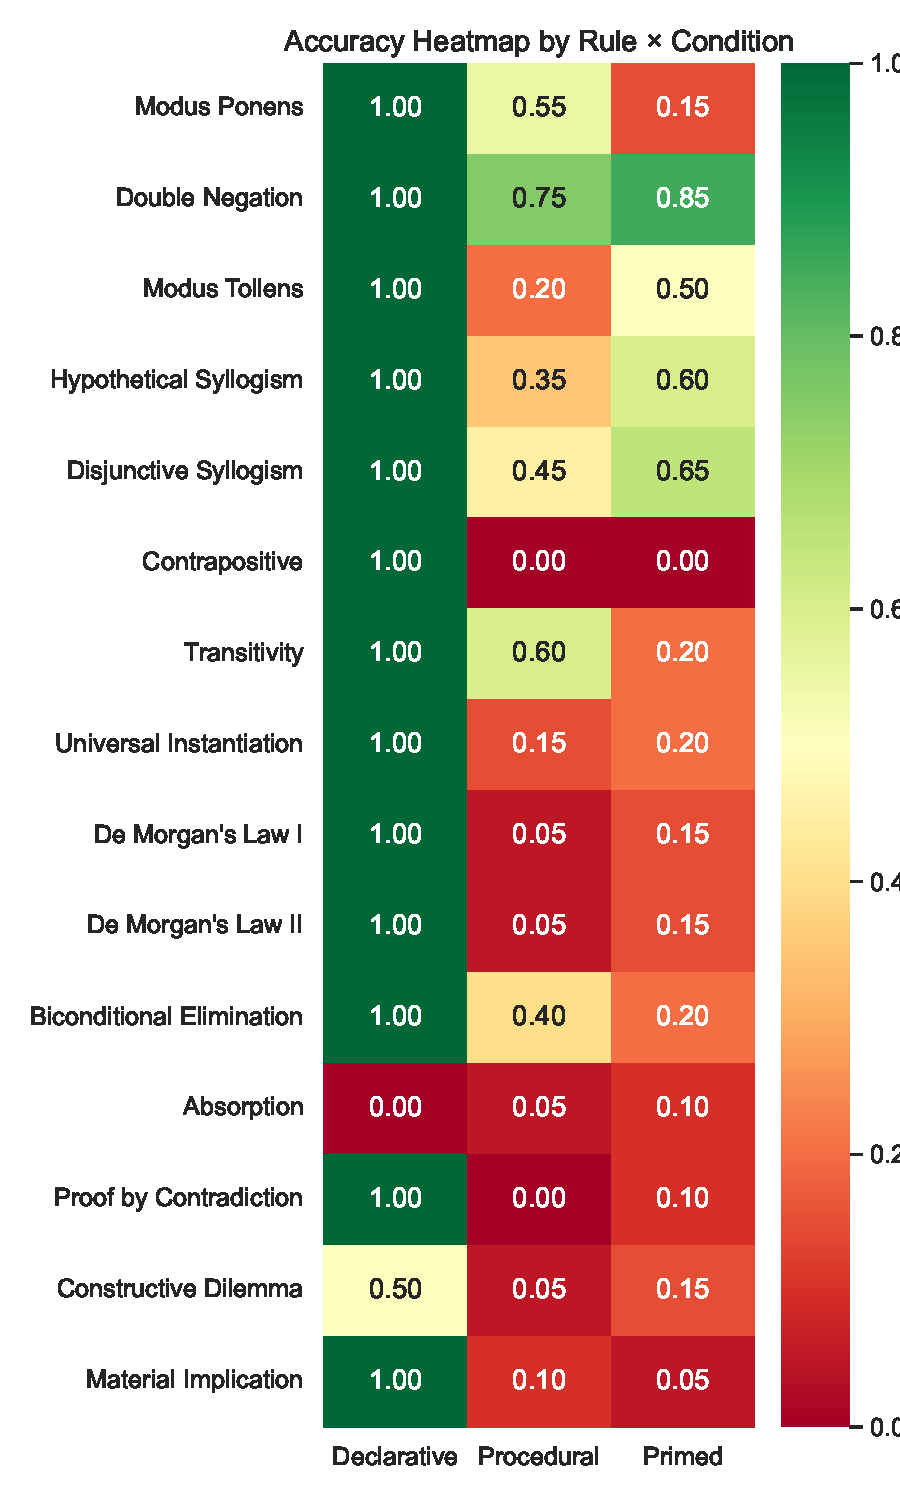
\includegraphics[width=0.7\columnwidth]{results/heatmap.pdf}
\caption{Accuracy heatmap: 15 rules $\times$ 3 conditions.}
\label{fig:heatmap_colm}
\end{figure}

\section{Example Problems and Responses}
\label{app:examples}

\paragraph{Example 1: Modus Ponens (C=1) --- Success.}
\begin{quote}
\small
\textbf{Problem:} If Kai studies hard, Kai will pass the exam. Kai studies hard. What can be concluded?\\
\textbf{Ground truth:} Kai will pass the exam.\\
\textbf{Declarative:} ``Modus Ponens: If P then Q; given P, conclude Q. Example: If it rains, the ground is wet\ldots'' \textbf{Score: 1.0}\\
\textbf{Procedural:} ``Since Kai studies hard and this implies passing, Kai will pass the exam.'' \textbf{Score: 1.0}\\
\textbf{Primed:} ``Applying Modus Ponens: P = `Kai studies hard', Q = `Kai passes'. P is true, so Q follows.'' \textbf{Score: 1.0}
\end{quote}

\paragraph{Example 2: Material Implication (C=4) --- D-P Gap.}
\begin{quote}
\small
\textbf{Problem:} We know that ``if the reactor overheats, the alarm sounds'' is equivalent to what disjunctive statement?\\
\textbf{Ground truth:} Either the reactor does not overheat, or the alarm sounds.\\
\textbf{Declarative:} ``Material Implication rewrites $P \to Q$ as $\neg P \lor Q$\ldots'' \textbf{Score: 1.0}\\
\textbf{Procedural:} ``If the reactor overheats, the alarm sounds. So the alarm sounds when overheating occurs.'' \textbf{Score: 0.0} (restated conditional, did not convert to disjunction)\\
\textbf{Primed:} ``Using material implication: $\neg$(`reactor overheats') $\lor$ (`alarm sounds') = `Either the reactor does not overheat or the alarm sounds.'\,'' \textbf{Score: 1.0}
\end{quote}

\paragraph{Example 3: Proof by Contradiction (C=4) --- Binding failure.}
\begin{quote}
\small
\textbf{Problem:} Assume $\sqrt{2}$ is rational. This leads to a contradiction. What can be concluded?\\
\textbf{Ground truth:} $\sqrt{2}$ is irrational.\\
\textbf{Declarative:} ``Proof by contradiction: assume $\neg P$, derive $\bot$, conclude $P$\ldots'' \textbf{Score: 1.0}\\
\textbf{Procedural:} ``Assuming $\sqrt{2}$ is rational leads to $p^2 = 2q^2$, so both p and q are even, contradicting the assumption they share no factors. Therefore $\sqrt{2}$ is irrational.'' \textbf{Score: 1.0}\\
\textbf{Primed:} ``The assumption that $\sqrt{2}$ is rational leads to a contradiction. By proof by contradiction, $\sqrt{2}$ must be irrational.'' \textbf{Score: 0.5} (correct conclusion but incomplete reasoning)
\end{quote}

\end{document}
